\documentclass[11pt]{article}
\usepackage{geometry,marginnote} % Pour passer au format A4
\geometry{hmargin=1cm, vmargin=1.5cm} % 

% Page et encodage
\usepackage[T1]{fontenc} % Use 8-bit encoding that has 256 glyphs
\usepackage[english,french]{babel} % Français et anglais
\usepackage[utf8]{inputenc} 

\usepackage{lmodern}
\usepackage[np]{numprint}
\setlength\parindent{0pt}

% Graphiques
\usepackage{graphicx,float,grffile}
\usepackage{tikz,pst-eucl,pst-plot,pstricks,pst-node,pstricks-add,pst-fun,pgfplots} 

% Maths et divers
\usepackage{amsmath,amsfonts,amssymb,amsthm,verbatim,scratch3}
\usepackage{multicol,enumitem,url,eurosym,gensymb,tabularx}

\DeclareUnicodeCharacter{20AC}{\euro}



% Sections
\usepackage{sectsty} % Allows customizing section commands
\allsectionsfont{\centering \normalfont\scshape}

% Tête et pied de page
\usepackage{fancyhdr} \pagestyle{fancy} \fancyhead{} \fancyfoot{}

%\fancyfoot[L]{Collège Faubert}
%\fancyfoot[C]{\thepage / 6}
%\fancyfoot[R]{Série Générale}

\renewcommand{\headrulewidth}{0pt} % Remove header underlines
%\renewcommand{\footrulewidth}{0pt} % Remove footer underlines

\newcommand{\horrule}[1]{\rule{\linewidth}{#1}} % Create horizontal rule command with 1 argument of height

\newcommand{\Pointilles}[1][3]{%
  \multido{}{#1}{\makebox[\linewidth]{\dotfill}\\[\parskip]
}}

\newtheorem{Definition}{Définition}

\usepackage{siunitx}
\sisetup{
    detect-all,
    output-decimal-marker={,},
    group-minimum-digits = 3,
    group-separator={~},
    number-unit-separator={~},
    inter-unit-product={~}
}

\setlength{\columnseprule}{1pt}


\begin{document}

\begin{center}
  \textit{Le plus grand ennemi de la connaissance n'est pas l'ignorance. C'est l'illusion de la connaissance.} 
  
  \textbf{Stephen Hawking}
\end{center}

\textbf{Ex : Calculer} 

\begin{multicols}{2} \begin{itemize}[label={$\bullet$}]
  \item $13 + 21 \times 35$ 
  \item $3 \times (13 + 21)$ 
  \item $(22 - 6) \times (5 + 35)$
  \item $52 \div 2 \times 5 + 131$
  \item $(13 + 6) \times (4 + 22) \times (17 - 9)$
  \item $154 + 22 \div 2 - 13 + 4 \times 23$
  \item $2 \times ( 5 + 3 \times (6 + 10))$
\end{itemize} \end{multicols}


\begin{figure}[H]
  \centering
  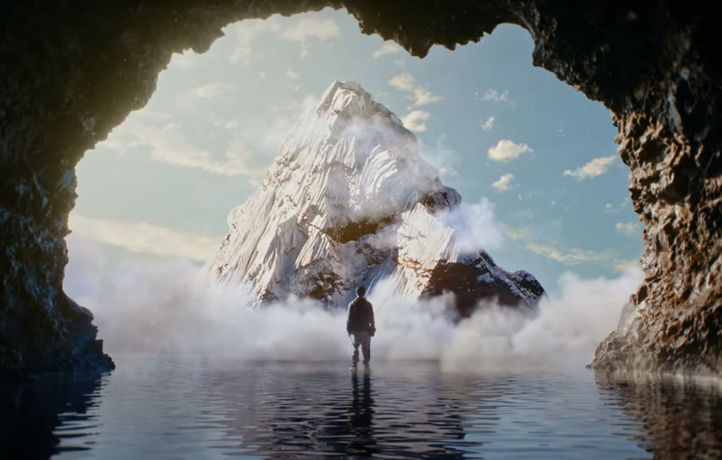
\includegraphics[width=0.4\linewidth]{5x1-calcul-numerique/kaizen.jpg}
\end{figure}

\textbf{pb1 : altitude} \\

L'Himalaya est la plus haute chaîne de montagne du monde. Son plus haut sommet est le mont Everest. Il culmine à une altitude de $8\,849$m. Inox et son équipe se préparent au camp de base situé à $5\,204$m d'altitude. Quelle altitude vont-ils devoir à gravir ? \\


\textbf{pb2 : distance} \\
 
Toujours au camp de base, le sherpa Manish note les distances qu'ils ont encore à parcourir jusqu'au sommet. 

\begin{multicols}{2}

\begin{figure}[H]
  \centering
  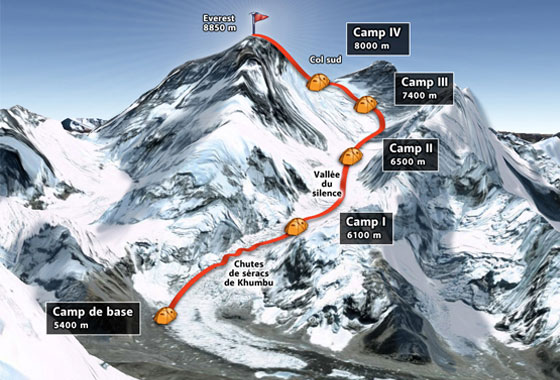
\includegraphics[width=0.8\linewidth]{5x1-calcul-numerique/camp.jpg}
\end{figure} \columnbreak

\begin{itemize}[label={$\bullet$}]
  \item Distance entre le camp de base et le camp 1 : $5$km \\
  \item Distance entre le camp 1 et le camp 2 : $4,2$km \\
  \item Distance entre le camp 2 et le camp 3 : $3,6$km \\
  \item Distance entre le camp 3 et le camp 4 : $4,8$km \\
  \item Distance entre le camp 4 et le sommet : $3$km \\
\end{itemize} 

\end{multicols}

\begin{enumerate}
  \item[1.] Quelle est la distance à parcourir entre le camp de base et le sommet ?
  \item[2.] Mathis rappelle à Inox qu'une fois au sommet, ils vont devoir redescendre jusqu'au camp de base. Quelle est la distance aller-retour ? \\
\end{enumerate}

\textbf{pb3 : coût} \\

Pour une ascension dans l’Himalaya et pour gravir l’Everest, il faut compter environ $50\,000$€ par personne entre les billets d'avion, le matériel et le permis. Il faut également payer des sherpa $8\,000$€. Afin de réaliser le documentaire, Inox a compté 6 accompagnants en plus de lui et 9 sherpa. Quel est le prix de son documentaire ?

\newpage

\begin{center}
  \textit{Le plus grand ennemi de la connaissance n'est pas l'ignorance. C'est l'illusion de la connaissance.} 
  
  \textbf{Stephen Hawking}
\end{center}

\textbf{Ex : Calculer} 

\begin{multicols}{2} \begin{itemize}[label={$\bullet$}]
  \item $14 + 21 \times 35$ 
  \item $4 \times (13 + 21)$ 
  \item $(20 - 6) \times (5 + 35)$
  \item $62 \div 2 \times 5 + 131$
  \item $(17 + 6) \times (4 + 22) \times (17 - 9)$
  \item $174 + 22 \div 2 - 13 + 4 \times 21$
  \item $4 \times ( 5 + 3 \times (6 + 10))$
\end{itemize} \end{multicols}


\begin{figure}[H]
  \centering
  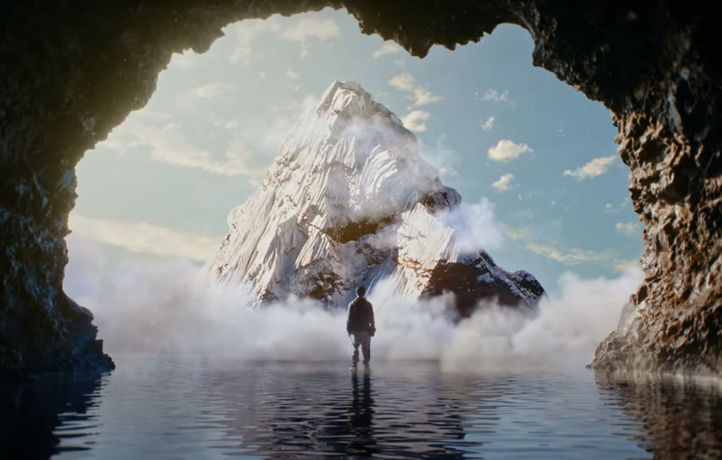
\includegraphics[width=0.4\linewidth]{5x1-calcul-numerique/kaizen.jpg}
\end{figure}

\textbf{pb1 : altitude} \\

L'Himalaya est la plus haute chaîne de montagne du monde. Son plus haut sommet est le mont Everest. Il culmine à une altitude de $8\,849$m. Inox et son équipe se préparent au camp de base situé à $5\,156$m d'altitude. Quelle altitude vont-ils devoir à gravir ? \\


\textbf{pb2 : distance} \\
 
Toujours au camp de base, le sherpa Manish note les distances qu'ils ont encore à parcourir jusqu'au sommet. 

\begin{multicols}{2}

\begin{figure}[H]
  \centering
  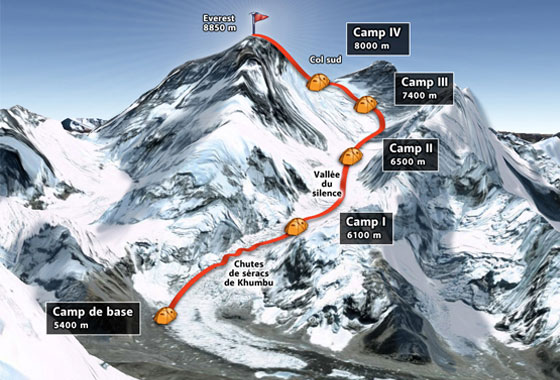
\includegraphics[width=0.8\linewidth]{5x1-calcul-numerique/camp.jpg}
\end{figure} \columnbreak

\begin{itemize}[label={$\bullet$}]
  \item Distance entre le camp de base et le camp 1 : $5$km \\
  \item Distance entre le camp 1 et le camp 2 : $4,1$km \\
  \item Distance entre le camp 2 et le camp 3 : $3,7$km \\
  \item Distance entre le camp 3 et le camp 4 : $4,7$km \\
  \item Distance entre le camp 4 et le sommet : $3$km \\
\end{itemize} 

\end{multicols}

\begin{enumerate}
  \item[1.] Quelle est la distance à parcourir entre le camp de base et le sommet ?
  \item[2.] Mathis rappelle à Inox qu'une fois au sommet, ils vont devoir redescendre jusqu'au camp de base. Quelle est la distance aller-retour ? \\
\end{enumerate}

\textbf{pb3 : coût} \\

Pour une ascension dans l’Himalaya et pour gravir l’Everest, il faut compter environ $50\,000$€ par personne entre les billets d'avion, le matériel et le permis. Il faut également payer des sherpa $8\,000$€. Afin de réaliser le documentaire, Inox a compté 7 accompagnants en plus de lui et 8 sherpa. Quel est le prix de son documentaire ?


\newpage

\begin{center}
  \textit{Le plus grand ennemi de la connaissance n'est pas l'ignorance. C'est l'illusion de la connaissance.} 
  
  \textbf{Stephen Hawking}
\end{center}

\textbf{Ex : Calculer} 

\begin{multicols}{2} \begin{itemize}[label={$\bullet$}]
  \item $16 + 21 \times 35$ 
  \item $6 \times (13 + 21)$ 
  \item $(24 - 6) \times (5 + 35)$
  \item $42 \div 2 \times 5 + 131$
  \item $(18 + 6) \times (4 + 22) \times (18 - 9)$
  \item $164 + 22 \div 2 - 13 + 4 \times 23$
  \item $5 \times ( 5 + 3 \times (6 + 12))$
\end{itemize} \end{multicols}


\begin{figure}[H]
  \centering
  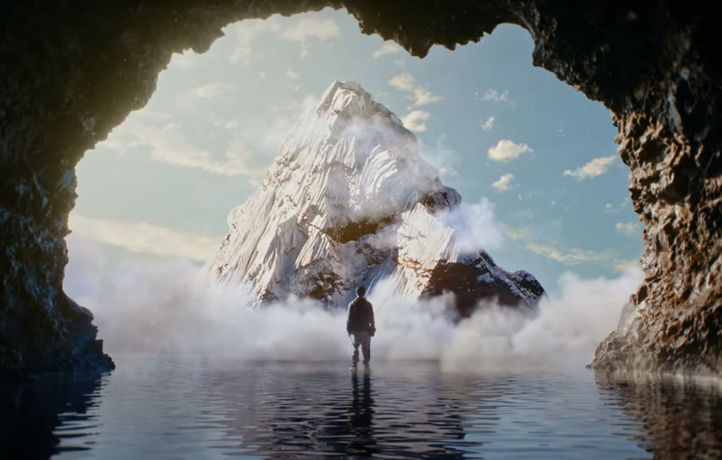
\includegraphics[width=0.4\linewidth]{5x1-calcul-numerique/kaizen.jpg}
\end{figure}

\textbf{pb1 : altitude} \\

L'Himalaya est la plus haute chaîne de montagne du monde. Son plus haut sommet est le mont Everest. Il culmine à une altitude de $8\,849$m. Inox et son équipe se préparent au camp de base situé à $5\,186$m d'altitude. Quelle altitude vont-ils devoir à gravir ? \\


\textbf{pb2 : distance} \\
 
Toujours au camp de base, le sherpa Manish note les distances qu'ils ont encore à parcourir jusqu'au sommet. 

\begin{multicols}{2}

\begin{figure}[H]
  \centering
  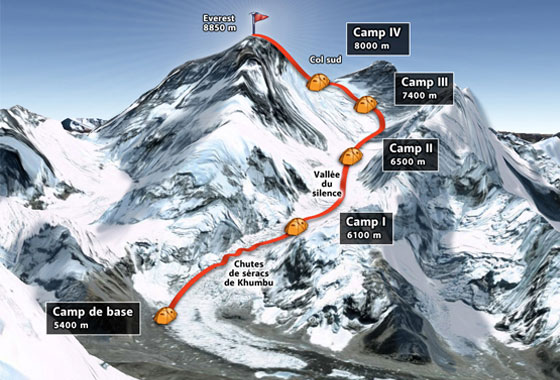
\includegraphics[width=0.8\linewidth]{5x1-calcul-numerique/camp.jpg}
\end{figure} \columnbreak

\begin{itemize}[label={$\bullet$}]
  \item Distance entre le camp de base et le camp 1 : $5$km \\
  \item Distance entre le camp 1 et le camp 2 : $4,3$km \\
  \item Distance entre le camp 2 et le camp 3 : $3,7$km \\
  \item Distance entre le camp 3 et le camp 4 : $4,9$km \\
  \item Distance entre le camp 4 et le sommet : $3$km \\
\end{itemize} 

\end{multicols}

\begin{enumerate}
  \item[1.] Quelle est la distance à parcourir entre le camp de base et le sommet ?
  \item[2.] Mathis rappelle à Inox qu'une fois au sommet, ils vont devoir redescendre jusqu'au camp de base. Quelle est la distance aller-retour ? \\
\end{enumerate}

\textbf{pb3 : coût} \\

Pour une ascension dans l’Himalaya et pour gravir l’Everest, il faut compter environ $50\,000$€ par personne entre les billets d'avion, le matériel et le permis. Il faut également payer des sherpa $8\,000$€. Afin de réaliser le documentaire, Inox a compté 7 accompagnants en plus de lui et 11 sherpa. Quel est le prix de son documentaire ?


\end{document}